\chapter[Learning Dynamical Systems via OT and Gradient Flows]{Learning Dynamical Systems via Optimal Transport and Gradient Flows}
\label{cha:neural_pde}

\dictum[Andrey Kolmogorov, \textit{\"Uber die analytischen Methoden in der Wahrscheinlichkeitsrechnung} (1931)]{%
  Ein solches mathematisch-definierbares System ist \"uberhaupt nicht die Wirklichkeit selbst, sondern nur ein Schema, welches zur Beschreibung der Wirklichkeit dienen kann.} % This mathematically defined system is not a reality itself, but a scheme that can be used to describe reality. From: On Analytical Methods in the Theory of Probability

% Introduction

\begin{figure}[t]
    \centering
    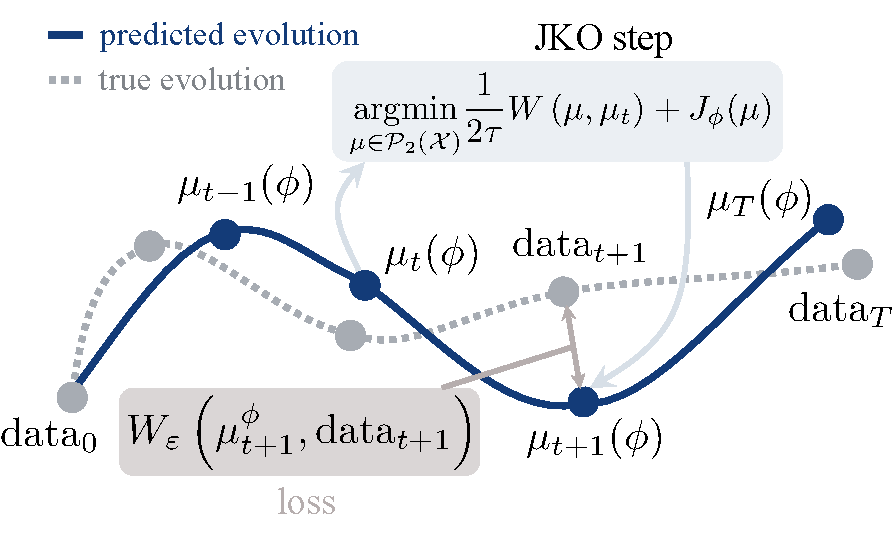
\includegraphics[width=.9\linewidth]{figures/fig_overview_jkonet.pdf}
    \caption{Given an observed trajectory $(\mu_0,\dots,\mu_T)$ of point clouds (gray), we seek parameters $\xi$ for the energy $J_\xi$ such that the predictions $\rho_1, \dots, \rho_T$ (blue) following a JKO flow from $\rho_0=\mu_0$ are close the observed trajectory (gray), by minimizing (as a function of $\xi$) the sum of Wasserstein distances between $\rho_{t+1}$, the JKO step from $\rho_{t-1}$ using $J_\xi$, and data $\mu_{t+1}$.}
    \label{fig:overview}
\end{figure}

\paragraph{Modeling Particle Dynamics as a JKO Scheme.} In this paper, we draw inspiration from both approaches above---the intuition from the recent NF literature that flows should mimic an optimal transport (OT as prior), and be able, through training, to predict future configurations (OT as a loss)---to propose a causal model for population dynamics. Our approach relies on a powerful hammer: the Jordan-Kinderlehrer-Otto (JKO) flow~\citep{jordan1998variational}, widely regarded as one of the most influential mathematical breakthroughs in recent history. While the JKO flow was initially introduced as an alternative method to solve the Fokker-Planck partial differential equation (PDE), its flexibility can be showcased to handle more complex PDEs \cite[\S4.7]{santambrogio2017euclidean}, or even describe the gradient flows of non-differentiable energies that have no PDE representation.
On a purely mechanical level, a JKO step is to measures what the proximal step~\citep{combettes2011proximal} is to vectors: In a JKO step, particles move to decrease collectively an {\em energy} (a real-valued function defined on measures), yet remain close (in Wasserstein sense) to the previous configuration. Our goal in this paper is to treat JKO steps as parameterized modules, and fit their parameter (the energy function) so that its outputs agree repeatedly over time with observed data. 
This approach presents several challenges: While numerical approaches to solve JKO steps have been proposed in low dimensional settings~\citep{burger2010, carrillo2021primal, peyre2015entropic,benamou2016augmented}, scaling it to higher dimensions is an open problem. Moreover, minimizing a loss involving a JKO step w.r.t. energy requires not only solving the JKO problem, but also computing the (transpose) Jacobian of its output w.r.t. energy parameters.

% We wish to reconstruct that energy potential from observations, assuming each observations follows iteratively a JKO flow.

\paragraph{Contributions.}\hspace{1em} Our contributions are two-fold. First, we propose a method, given an input configuration and an energy function, to compute JKO steps using input convex neural networks (ICNN)~\citep{amos2017input,makkuva2020optimal} (see also concurrent works that have proposed similar approaches~\citep{alvarez2021optimizing, mokrov2021large}). Second, we view the JKO step as an inner layer, a \textsc{JKOnet} module parameterized by an energy function, which is tasked with moving the particles of an input configuration along an OT flow (the gradient of an optimal ICNN), trading off a lower energy with proximity to the previous configuration.
%This module, \textsc{JKOnet}, can be therefore seen as a parameterized \emph{mover} of particles that is constrained by design to produce locally (OT) optimal displacements. 
We propose to estimate the parameters of the energy by minimizing a fitting loss %(as a function of the energy itself) 
computed between the outputs of the \textsc{JKOnet} module (the prediction) and the ground truth displacements, as illustrated in Figure~\ref{fig:overview}.
We demonstrate \textsc{JKOnet}'s range of applications by applying in on synthetic potential- and trajectory-based population dynamics, as well as developmental trajectories of human embryonic stem cells based on single-cell genomics data.


\section[On the Connection between OT and Fokker-Planck Equations]{On the Connection between Optimal Transport and Fokker-Planck Equations}

\paragraph{JKO Flows.}
In their seminal paper, \citet{jordan1998variational} study diffusion processes under the lens of the OT metric \citep[see also][]{ambrosio2006gradient} and introduce a scheme that is now known as the JKO flow: Starting with $\rho_0$, and given a real-valued energy function $J:\mathcal{P}(\mathbb{R}^d)\rightarrow \mathbb{R}$ driving the evolution of the system, they define iteratively for $t\geq 0$, :
\begin{equation} \label{eq:jko}
    \rho_{t+1} = \arg \min_{\rho\in \mathcal{P}_2(\mathbb{R}^d)} J(\rho) + \frac{1}{2\tau} W^2(\rho, \rho_{t})\,,
\end{equation}
where $\tau$ is a time step parameter. These successive minimization problems result in a sequence of probability measures in $\mathcal{P}(\mathbb{R}^d)$. The JKO flow can thus be seen as the analogy of the usual proximal descent scheme, tailored for probability measures~\citep[p.285]{santambrogio2015optimal}. \citet{jordan1998variational} show that as step size $\tau \rightarrow 0$, and for a specific energy $J$ that is the sum of a linear term and the negentropy, the measures describing the JKO flow recover solutions to a Fokker-Planck equation. In this work, following in the footsteps of more general applications of the JKO scheme~\citep[\S4.8]{santambrogio2017euclidean}, we model dynamics without necessarily having in mind PDE solutions in mind, to interpret instead the JKO step as a more general parametric type of dynamic for probability measures, exclusively parameterized by the energy $J$ itself.


\section{\textsc{JKOnet}: A Proximal Optimal Transport Model} 

Given $T$ discrete measures $\mu_0, \dots, \mu_T$ describing the time evolution of a population, we posit that such an evolution follows a JKO flow for the free energy functional $J$, and assume that energy does not change throughout the dynamic. We parameterize the energy $J$ as a neural network with parameters $\xi$, and fit $\xi$ so that the JKO flow model matches the observed data. 

Fitting parameter $\xi$ with a reconstruction loss requires, using the chain rule, being able to differentiate the JKO step's output w.r.t. $\xi$ (see Fig.~\ref{fig:overview}), and more precisely provide a way to apply that transpose Jacobian to an arbitrary vector when using reverse-mode differentiation. To achieve this, we introduce a novel approach to numerically solve JKO flows using ICNNs (\S~\ref{sec:jko_icnn}), resulting in a bilevel optimization problem targeting the energy $J_\xi$ (\S~\ref{sec:learn_energy}).

\subsection{Reformulation of JKO Flows via ICNNs} \label{sec:jko_icnn}
Given a starting condition $\rho_t$ and energy functional $J_\xi$, the JKO step consists in producing a new measure $\rho_{t+1}$ implicitly defined as the minimizer of~\eqref{eq:jko}. Solving directly~\eqref{eq:jko} on the space of measures, involves substantial computational costs. Different numerical schemes have been developed, e.g., based notably on Eulerian discretization of measures \citep{carrillo2021primal, benamou2016}, and/or entropy-regularized optimal transport \citep{peyre2015entropic}. However, these methods are limited to small dimensions since the cost of discretizing such spaces grows exponentially. Except for the Eulerian approach proposed in \citep{peyre2015entropic}, obtained as the fixed point of a Sinkhorn type iteration, the differentiation would also prove extremely challenging as a function of the energy parameter $\xi$.

\looseness=-1 To reach scalability and differentiability, we build upon the approach outlined in \citet{benamou2016} to reformulate the JKO scheme as a problem solved over convex functions, rather than on measures $\rho$. Effectively, this is equivalent to making a change of variables in~\eqref{eq:jko}: Introduce a (variable) convex function $\psi$, and replace the variable $\rho$ by the variable $\nabla \psi_{\#}\rho_t$. Writing
\begin{equation}\label{eq:en}
\begin{split}
\mathcal{E}_J(\rho, \nu) := J(\rho) +\frac{1}{2 \tau}W_2^2(\rho, \nu),\\
\end{split}
\end{equation}
this identity states that, assuming $\mu$ and $\nu$ being absolutely continuous w.r.t. Lebesgue measure that
$$\min_{\rho}\mathcal{E}_J(\rho,\nu) = \min_{\psi \text{ convex}} \mathcal{F}_J(\psi, \nu):= \mathcal{E}_J(\nabla \psi_{\#}\nu, \nu)\,,$$
simplifying the Wasserstein term in \eqref{eq:en}, using the assumption that $\psi$ is convex and \citeauthor{Brenier1987}'s theorem (\S~\ref{sec:intro}):
\begin{equation}\mathcal{F}_J(\psi, \nu) = J(\nabla \psi_{\#}\nu) +\frac{1}{2 \tau} \!\! \int\!\! \| x - \nabla \psi(x) \|^2 d \nu(x)\label{eq:JKO_psi}
\end{equation}

We pick an ICNN architecture to optimize over a restricted family of convex functions, $\{\psi_{\theta}\}$, and define, starting from $\rho_0(\xi):=\mu_0$, the recursive sequence for $t\geq 0$,
\begin{equation} \label{eq:next_pop}
\rho_{t+1}(\xi) := \nabla \psi_{\theta^\star\!(\xi, \rho_t(\xi))\, \#}\, \rho_{t}(\xi)\,,
\end{equation}
with $\theta^\star(\xi, \rho_t)$ defined implicitly using $\xi$ and any $\nu$ as 
\begin{align} \label{eq:thetastar}
    \theta^\star(\xi, \nu):=\arg \min_{\theta} \mathcal{F}_J(\psi_{\theta},\nu)
\end{align}

\vspace{-20pt} \paragraph{Strong Convexity of $\psi_\theta$.} The strong convexity and smoothness of a potential $\psi$ impacts the regularity of the corresponding OT map $\nabla\psi$ ~\citep{caffarelli2000monotonicity,figalli2010optimal}, since one can show that for a $\ell$-strongly convex, $L$-smooth $\psi$ one has~\citep{paty2020regularity} that
$$
\ell \|x - y\| \leq \|\nabla\psi(x) -\nabla\psi(y)\|  \leq L\|x - y\|.
$$
While it is more difficult to enforce the $L$-smoothness of a neural network, and more generally its Lipschitz constants \citep{scaman2018lipschitz} it is easy to enforce its strong convexity, by simply adding a term $\ell \|x\|^2/2$ to the corresponding potential, or a residual rescaled term $\ell x$ to the output $\nabla\psi(x)$. This approach can be used to enforce that the push-forward of the gradient of an ICNN does not collapse to a single point, maintaining spatial diversity.

\subsection{Learning the Free Energy Functional}  \label{sec:learn_energy}
The energy function $J_\xi : \mathcal{P}(\mathbb{R}^d) \rightarrow \mathbb{R}$ can be any parameterized function taking a measures as an input. 
Since our model assumes that the observed dynamic is parameterized entirely by that energy (and the initial observation $\rho_0$), the more complex this dynamic, the more complex one would expect the energy $J_\xi$ to be. We focus in this first attempt on linear functions in the space of measures, that is expectations over $\rho$ of a vector-input neural network $E_\xi$
\begin{equation} \label{eq:energy}
    J_\xi(\rho) := \int E_\xi(x) d\rho(x),
\end{equation}
where $E_\xi:\mathbb{R}^d \rightarrow \mathbb{R}$ is a multi-layer perceptron (MLP).

\begin{algorithm}[t]
\KwIn{Dataset $\mathcal{D}=\{\{\mu_t^0 \}_{t=0}^T, \ldots, \{\mu_t^N \}_{t=0}^T\}$ of $N$ population trajectories, $\xi^0$ energy parameter initialization, $\theta^0$ ICNN parameter initialization, learning rates $\text{lr}_\theta$ and $\text{lr}_\xi$, step $\tau$, regularizer $\varepsilon$, tolerance $\alpha$, {\texttt{TeacherForcing}} flag.}
\KwOut{Free energy $J_{\xi}$ explaining underlying population dynamics of snapshot data.}
$\xi\leftarrow \xi^0$

\For{$\{\mu_t\}_{t=0}^T \in \mathcal{D}$} {
\For{$t \gets 0$ \textbf{to} $T-1$} {

  $\theta\leftarrow \theta^0$

  \If{\texttt{TeacherForcing}}{
    $\nu \leftarrow \mu_t$
  }
  \Else{$\nu \leftarrow \rho_t(\xi)$}
  \While{$\frac{\sum_i \norm{\nabla_{\theta_i}\mathcal{F}_{J_\xi}(\theta)}_2}{\sum_i \text{count}(\theta_i)} \ge \alpha$}{
    
    $\theta \leftarrow \theta - \text{lr}_\theta \times \nabla_\theta \mathcal{F}_{J_\xi,\nu}(\theta)$
  }
  $\rho_{t+1}(\xi) \leftarrow \nabla \psi_{\theta \#} \nu$

  $\xi \leftarrow \xi - \text{lr}_\xi \times \nabla_\xi \cW(\rho_{t+1}(\xi), \mu_{t+1})$
}
}
\Return{$J_{\xi}$}

\caption{\textsc{JKOnet} Algorithm.}
\label{algo:jkonet}
\end{algorithm}

\begin{figure}[H]
 \vspace{-10pt}
    \centering
    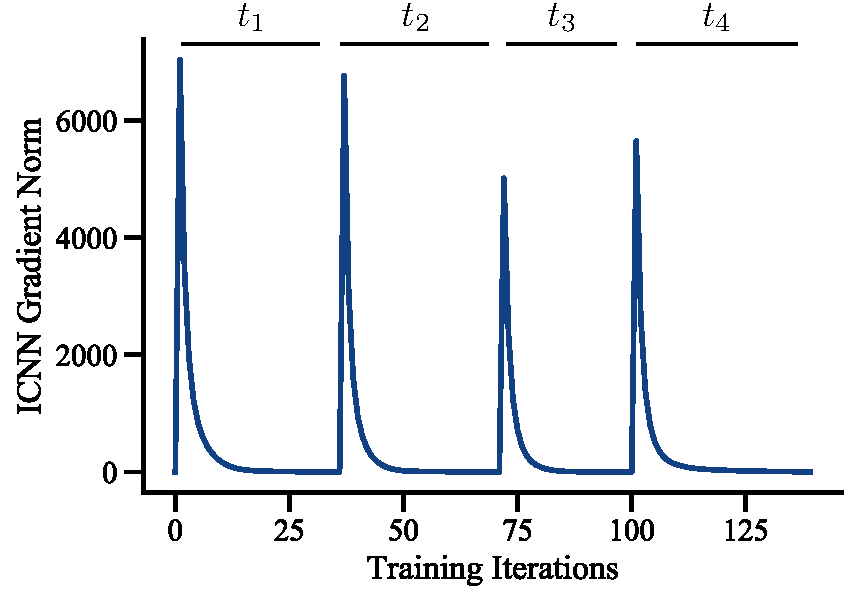
\includegraphics[width=.9\linewidth]{figures/fig_optimization_icnn.pdf}
    \caption{Optimization of the ICNN used in JKO steps. The bumps correspond to a change in the outer iteration, the smooth decrease in between correspond to a single minimization~\eqref{eq:thetastar} of a time step $t_i$. \vspace{-10pt}}
    \label{fig:training_icnn}
\end{figure}


Inferring nonlinear energies accounting for population growth and decline, as well as interactions between points, using the formalism of \citep{de2019stochastic}, transformers~\citep{vaswani2017attention} or set pooling methods \citep{edwards2016, zaheer2017}, is an exciting direction for future work.

To address slow convergence and instabilities for dynamics with many snapshots, we use teacher forcing \citep{williams1989learning} to learn $J_\xi$ through time. In those settings, during training, $J_\xi$ uses the ground truth as input instead of predictions from the previous time step. At test time, we do not use teacher forcing.

\begin{figure*}[ht]
\vspace{-10pt}
\centering
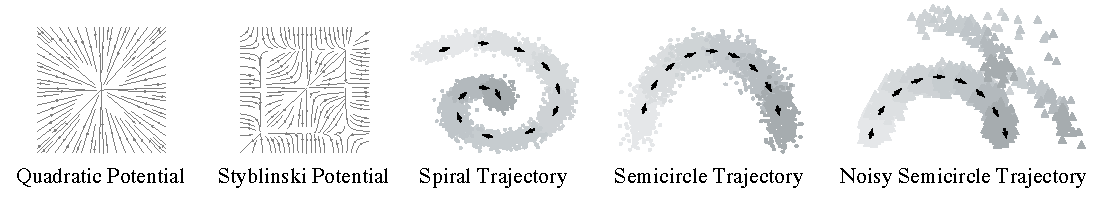
\includegraphics[width=1.0\textwidth]{figures/fig_task_overview_noise.pdf}
\caption{Overview on different tasks including trajectory- and potential-based dynamics.}
\label{fig:task_overview}
\end{figure*}

\begin{figure*}[h]
\vspace{-10pt}
\subfloat[\centering Quadratic Potential.]{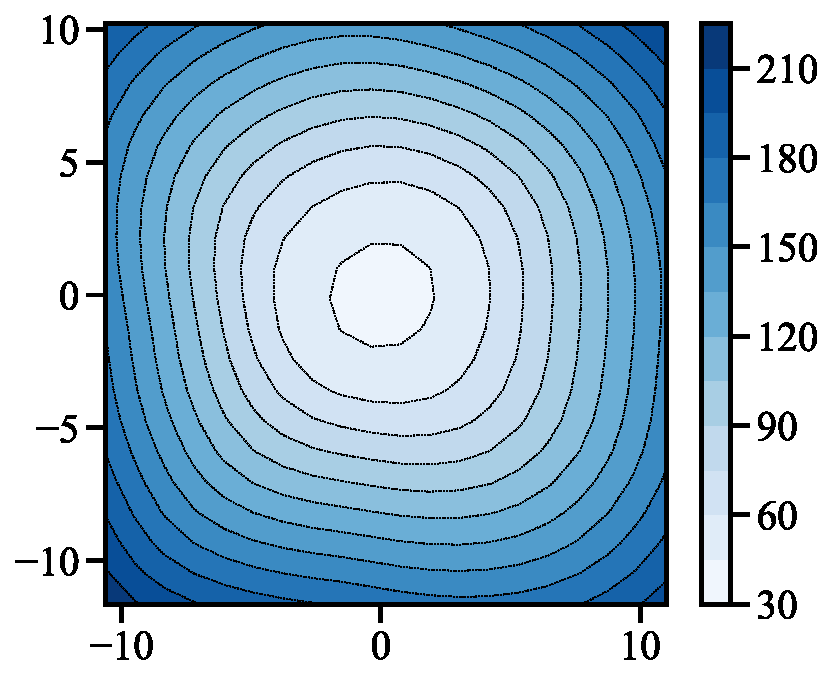
\includegraphics[width=.22\linewidth]{figures/fig_energy_implicit_quadratic.pdf}}
\subfloat[\centering Styblinski Potential.]{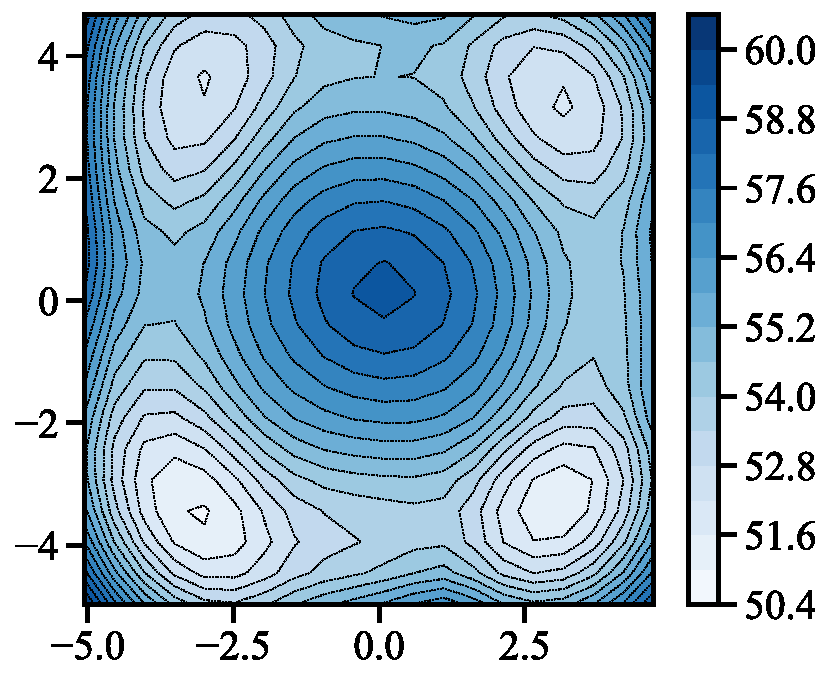
\includegraphics[width=.22\linewidth]{figures/fig_energy_implicit_styblinski.pdf}}
\subfloat[\centering Semicircle Trajectory \emph{with} teacher forcing.]{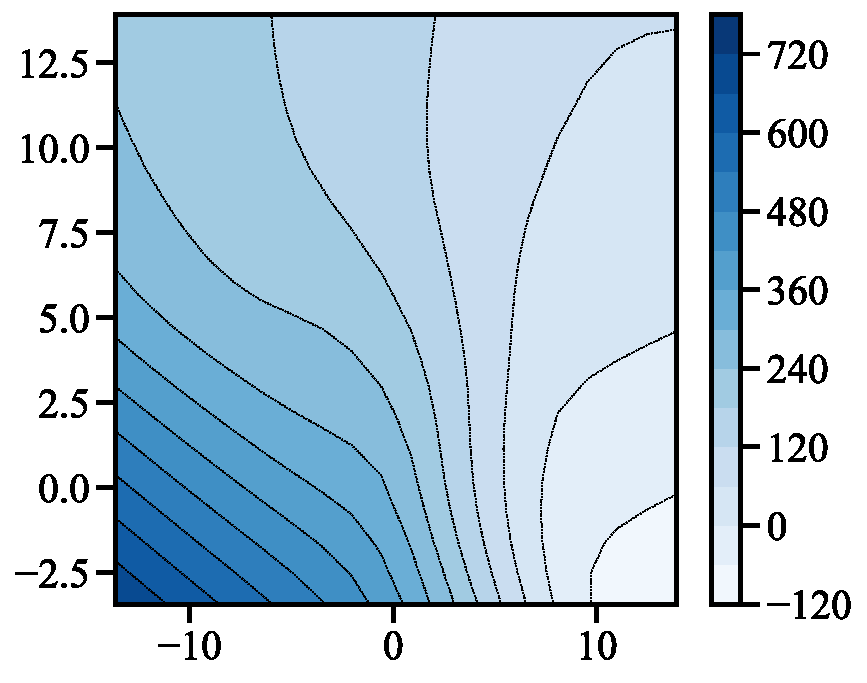
\includegraphics[width=.23\linewidth]{figures/fig_energy_implicit_semicircle_tf.pdf}}
\subfloat[\centering Predicted Population Evolution on Semicircle Trajectory.]{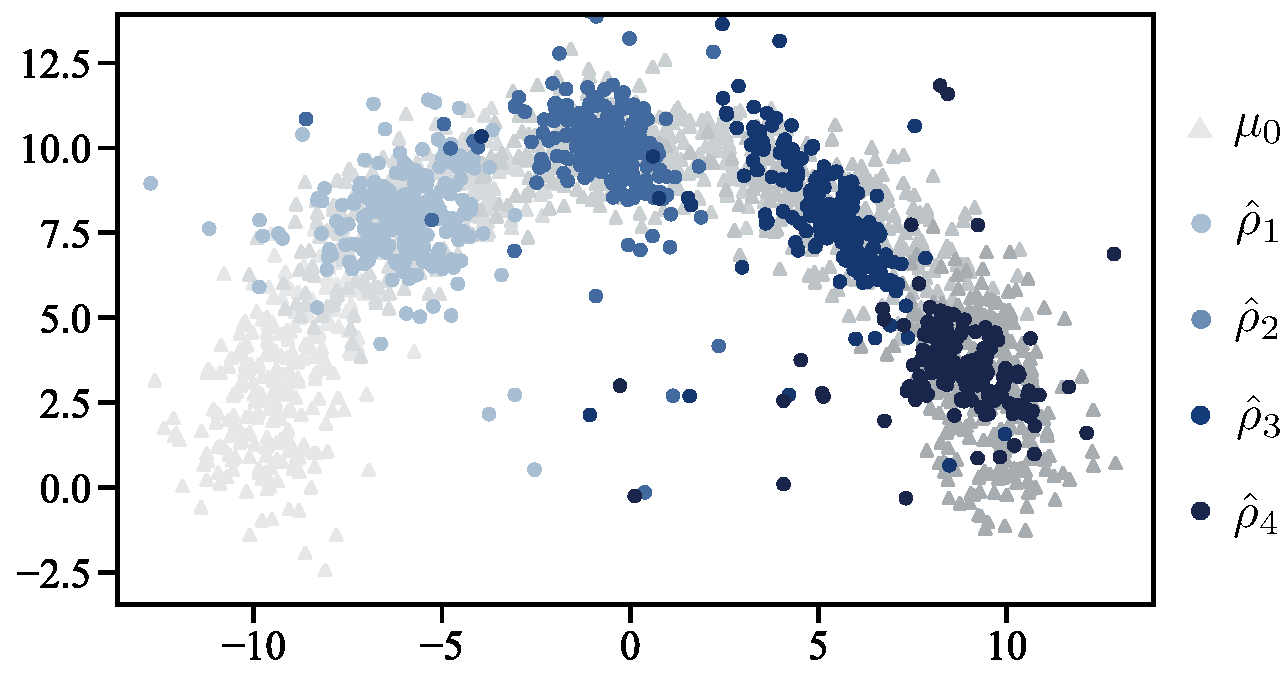
\includegraphics[width=.33\linewidth]{figures/fig_prediction_implicit_semicircle_tf.pdf}}
\caption{\textbf{Results of \text{JKOnet} on Potential- and Trajectory-based Dyanamics.} (a)-(c) Contour plots of the energy functionals $J_\xi$ of \textsc{JKOnet} on potential- and trajectory-based population dynamics in different training settings (i.e., trained with or without teacher forcing \S~ \ref{sec:learn_energy}), color gradients depict the magnitude of $J_\xi$. (d) Predicted population snapshots ($\hat{\rho}_1, \dots, \hat{\rho}_4$) (blue) and data trajectory ($\mu_0, \dots, \mu_4)$ (gray).}
\label{fig:exp_jkonet_pot_traj}
\end{figure*}

\subsection{Bilevel Formulation of \textsc{JKOnet}}
Learning the free energy functional $J_\xi$ while solving each JKO step via an ICNN results in a challenging bilevel optimization problem.
At each time step, the predicted dynamics are compared to the ground truth trajectory $(\mu_0, \mu_1, \dots, \mu_T)$ with a Sinkhorn loss \eqref{eq:sinkhorn},
\begin{align}\label{eq:fittingloss}
\begin{split}
    \min_\xi & \sum_{t=0}^{T-1} \cW(\rho_{t+1}(\xi), \mu_{t+1}), \\
    \text{s.t. } & \rho_{0}(\xi) := \mu_0, \\
      & \rho_{t+1}(\xi) := \nabla \psi_{\theta^\star\, \#}\, \rho_{t}(\xi)\,, \\
      & \theta^\star:=\arg \min_{\theta} \mathcal{F}_{J_{\xi}}(\psi_{\theta},\rho_t(\xi))
\end{split}
\end{align}
The dependence of the Sinkhorn divergence losses in \eqref{eq:fittingloss} on $\xi$ only appears in the fact that the predictions $\rho_{t+1}(\xi)$ are themselves implicitly defined as solving a JKO step parameterized with the energy $J_\xi$. 
Learning  $J_\xi$ through the exclusive supervision of data observations requires therefore to differentiate the arg-minimum of a JKO problem, down therefore through to the lower-level optimization of the ICNN. We achieve this by implementing a differentiable double loop in \texttt{JAX}, differentiating first the Sinkhorn divergence using the \texttt{OTT}\footnote{\href{https://github.com/ott-jax/ott}{github.com/ott-jax/ott}} package \citep{cuturi2022optimal}, and then backpropagating through the ICNN optimization by unrolling Adam steps \citep{kingma2014adam, metz2016unrolled, lorraine2020}.


\begin{figure*}[ht]
\subfloat[\centering \textsc{JKOnet} on 30\% corrupted data.]{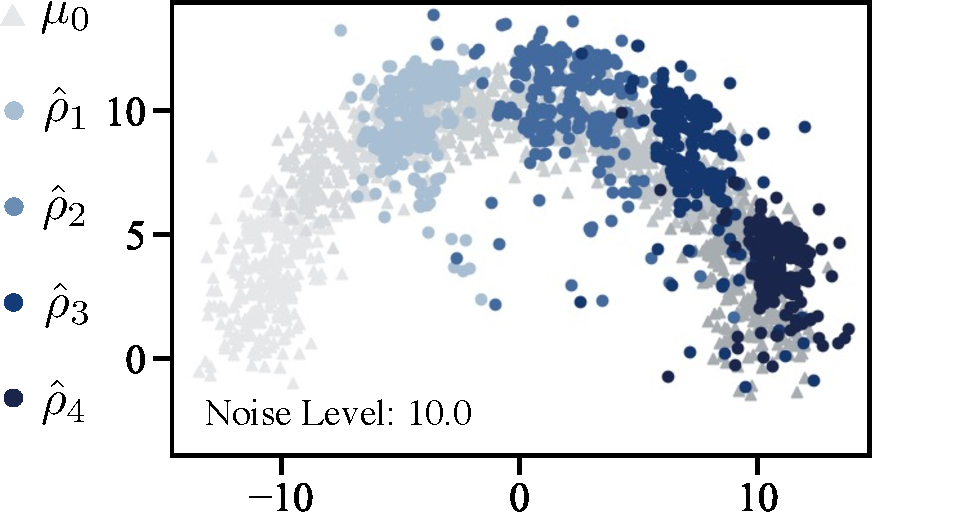
\includegraphics[width=.28\linewidth]{figures/fig_predictions_jko_noise.pdf}}
\subfloat[\centering Forward method on 30\% corrupted data.]{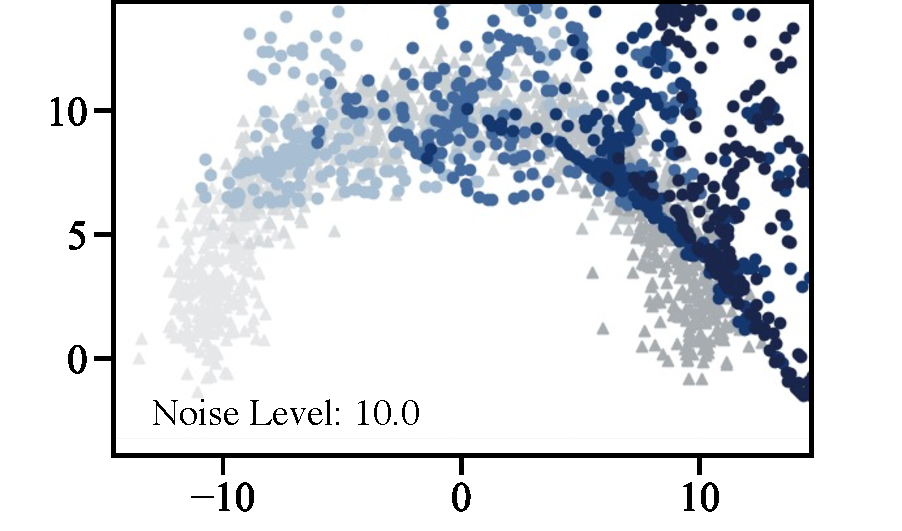
\includegraphics[width=.26\linewidth]{figures/fig_predictions_forward_noise.pdf}}
\subfloat[\centering $W_\epsilon$ \eqref{eq:reg-ot} vs. noise level on 20\% corrupted data.]{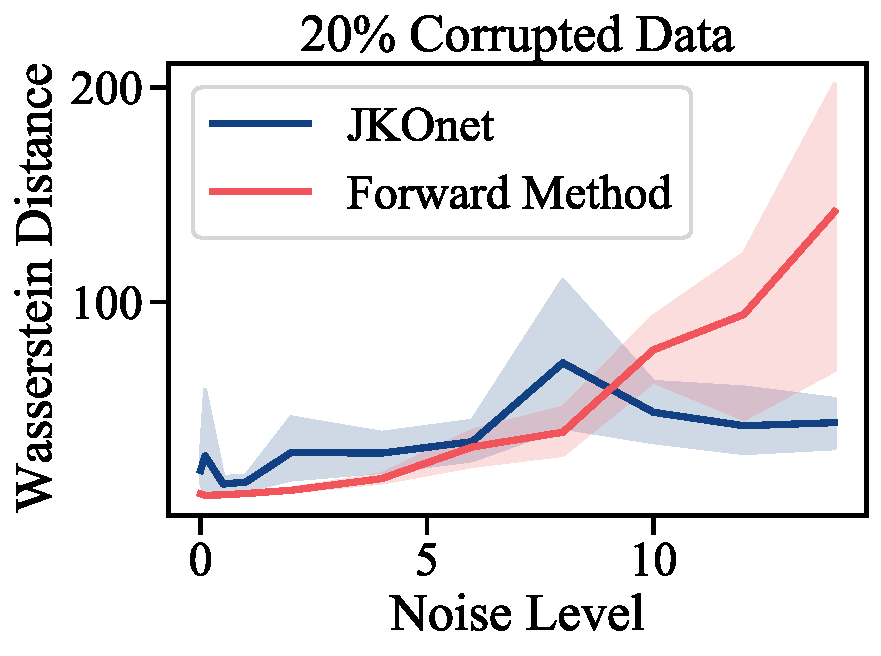
\includegraphics[width=.23\linewidth]{figures/fig_fb_comp_noise_20.pdf}}
\subfloat[\centering $W_\epsilon$ \eqref{eq:reg-ot} vs. noise level on 30\% corrupted data.]{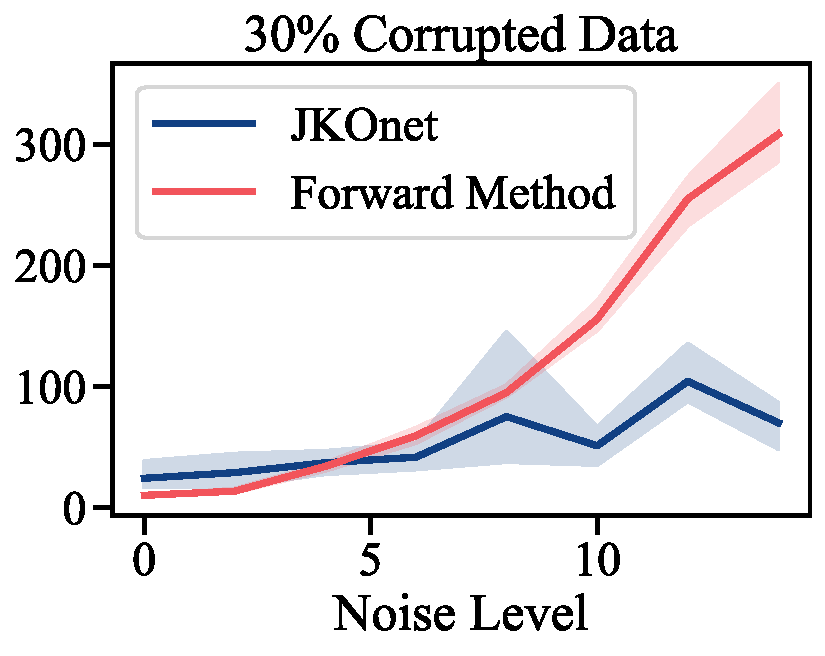
\includegraphics[width=.22\linewidth]{figures/fig_fb_comp_noise_30.pdf}}
\caption{Comparison between \textsc{JKOnet} and the forward method in settings of increasing noise on corrupted data on the semicircle trajectory task.}
\label{fig:exp_comp_noise}
\end{figure*}

\begin{figure*}[ht]
\subfloat[\centering Forward method, \protect\newline \emph{with} teacher forcing.]{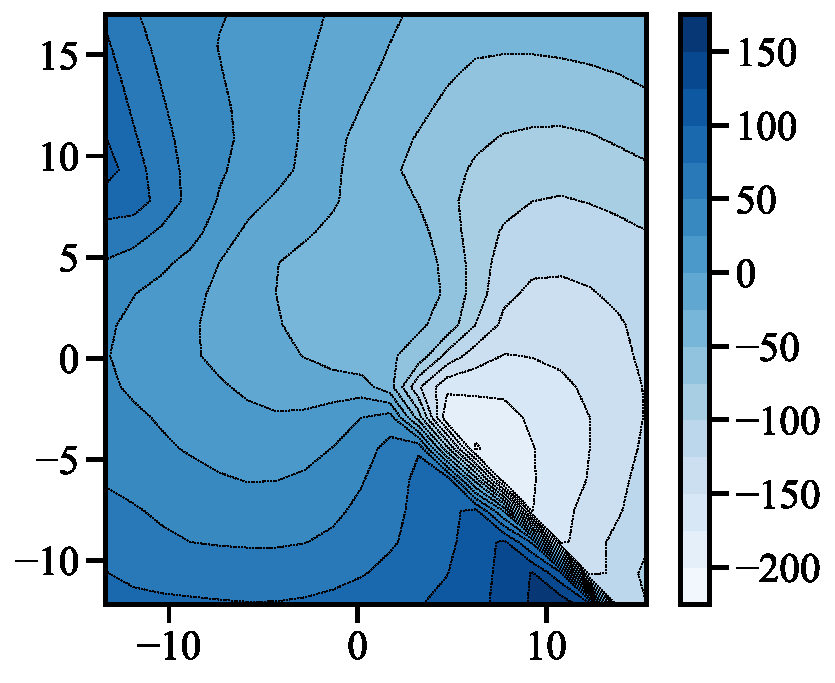
\includegraphics[width=.25\linewidth]{figures/fig_energy_explicit_spiral_tf.pdf}}
\subfloat[\centering Forward method, \protect\newline \emph{no} teacher forcing.]{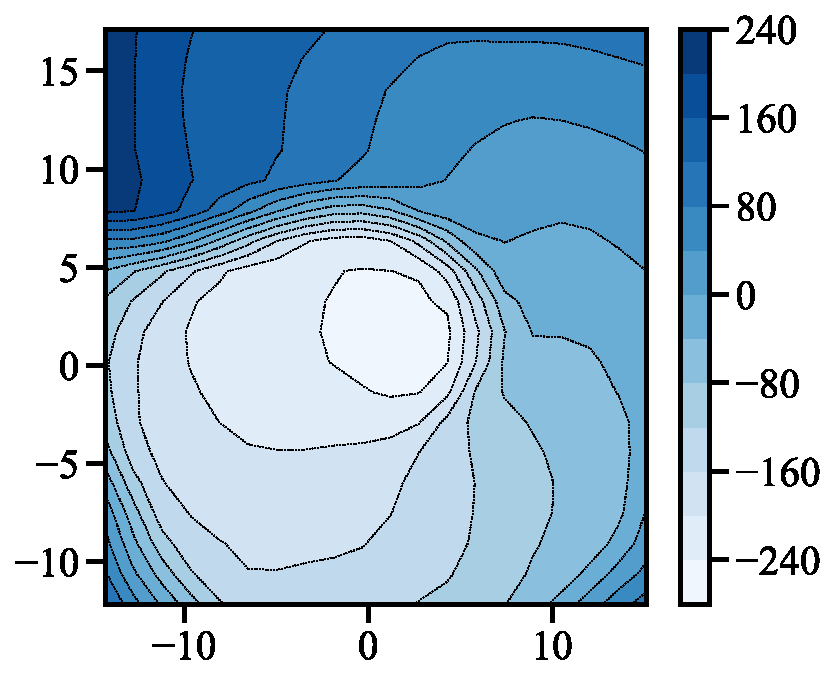
\includegraphics[width=.25\linewidth]{figures/fig_energy_explicit_spiral.pdf}}
\subfloat[\centering \textsc{JKOnet}, \protect\newline \emph{with} teacher forcing.]{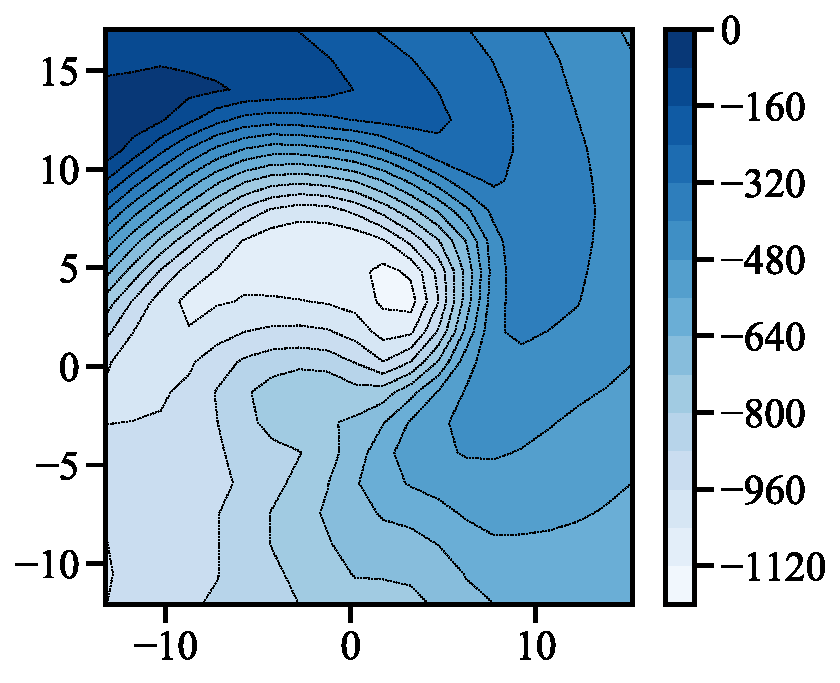
\includegraphics[width=.25\linewidth]{figures/fig_energy_implicit_spiral_tf.pdf}}
\subfloat[\centering \textsc{JKOnet}, \protect\newline \emph{no} teacher forcing.]{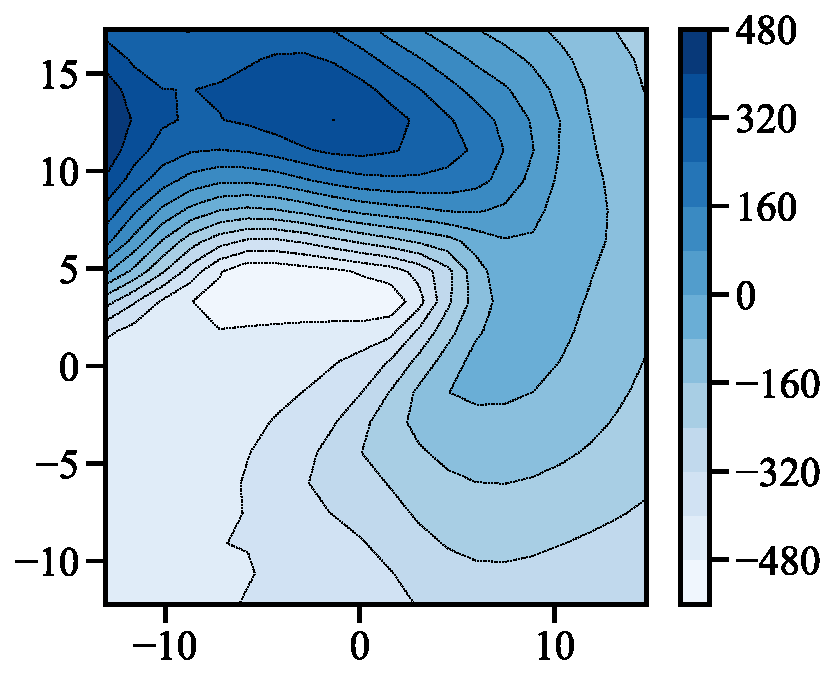
\includegraphics[width=.25\linewidth]{figures/fig_energy_implicit_spiral.pdf}}
\caption{Comparison between energy functionals $J_\xi$ of the spiral trajectory task (see \ref{fig:task_overview}) between the forward method and \textsc{JKOnet}, trained with or without teacher forcing \S~\ref{sec:learn_energy}). When using teacher forcing, the forward method overfits a gap on the lower-right corner of the spiral, outputting a highly irregular energy. When taking into account the entire trajectory recursively, the Forward method does better overall, but is unable to recover an energy as precise as that returned by \textsc{JKOnet}.}
\label{fig:exp_comp_spiral}
\end{figure*}

\newpage
\paragraph{Inner Loop Termination.} A question that arises when defining $\rho_{t+1}(\xi)$ lies in the budget of gradient steps needed or allowed to optimize the parameters $\theta$ of the ICNN, before taking a new gradient step on $\xi$ in the outer loss. A straightforward approach in \texttt{JAX} \citep{jax2018github} would be to use a preset number of iterations with a \texttt{for} loop (\texttt{jax.lax.scan}). 
We do observe, however, that the number of iterations needed to converge in relevant scenarios can vary significantly with the ICNN architecture and/or the hardness of the underlying task.
We propose to use instead a differentiable fixed-point loop to solve each JKO step up to a desired convergence threshold.
We measure convergence of the optimization of the ICNN via the average norm of the gradient of the JKO objective w.r.t. the ICNN parameters $\theta$, i.e., $\sum_i \norm{\nabla_{\theta_i}\mathcal{F}_{J_\xi}(\theta_i, \xi)}_2/\sum_i \text{count}(\theta_i)$.
We observe that this approach is robust across datasets and architectures of the ICNN. An exemplary training curve for the ICNNs updated successively along a time sequence is shown in Figure~\ref{fig:training_icnn}.

\paragraph{Reverse-Mode Differentiation.} The Jacobian $\partial \rho_{t+1} / \partial\xi$ arising when computing the gradient $\nabla_\xi \cW(\rho_{t+1}(\xi), \mu_{t+1})$ is obtained by unrolling the while loop above. The gradient term of the Sinkhorn divergence w.r.t the first argument is given by the Danskin envelope theorem \citep{danskin2012theory}.

% The Jacobian $\partial \rho^\xi_{t+1} / \partial\xi$ that appears when computing $\nabla_\xi \cW(\text{data}_{t+1}, \rho_{t+1}(\xi))$ is computed by unrolling the iterations of the while loop above.

\paragraph{Setting $\tau$ in \eqref{eq:JKO_psi}.} 
In usual JKO applications, $\tau$ needs to be tuned manually. In this work, the energy $J_\xi$ is not fixed, but trained to fit data. Since we put no constraints on the scaling of $J_\xi$, $\tau$ can be set to $1$ without loss of generality, as the parameter $\xi$ will automatically adjust so that the scale of $J_\xi$ induces steps of a relevant length to fit data. This only holds (as with a usual JKO step) if the trajectories are sampled regularly. For irregularly spaced time series, $\tau$ can be adapted at train and test time to the spacing of timestamps (shorter steps requiring larger $\tau$).


\begin{table*}[t]
    \caption{Evaluation of predictive performance w.r.t. the entropy-regularized Wasserstein distance $W_\varepsilon$ \eqref{eq:reg-ot} of \textsc{JKOnet} and the forward method on the embryoid body scRNA-seq data per time step (using 3 runs).}
    \label{tab:exp_jkonet_cell_pred}
    \centering
\adjustbox{max width=.75\linewidth}{%
    \begin{tabular}{lcccc}
    \toprule
         \textbf{Method} & \multicolumn{4}{c}{\textbf{Prediction Loss ($W_\varepsilon$})} \\
         \cmidrule{2-5}
         & Day 6 to 9 & Day 12 to 15 & Day 18 to 21 & Day 24 to 27 \\
    \midrule
    \textbf{One-Step Ahead} \\
        \tabindent Forward Method & $0.187 \pm 0.001$ & $0.162 \pm 0.010$ & $0.185 \pm 0.020$ & $0.203 \pm 0.004$ \\
        \tabindent \textsc{JKOnet} & $\bf{0.133 \pm 0.020}$ & $\bf{0.133 \pm 0.008}$ & $\bf{0.172 \pm 0.0130}$ & $\bf{0.169 \pm 0.004}$ \\
    \textbf{All-Steps Ahead} \\
        \tabindent Forward Method & $0.225 \pm 0.023$ & $0.160 \pm 0.001$ & $0.171 \pm 0.016$ & $0.183 \pm 0.007$ \\
        \tabindent \textsc{JKOnet} & $\bf{0.148 \pm 0.015}$ & $\bf{0.144 \pm 0.013}$ & $\bf{0.154 \pm 0.024}$ & $\bf{0.138 \pm 0.034}$ \\
    \bottomrule
    \end{tabular}
}
\end{table*}

\section{Empirical Evaluation} \label{sec:evaluation}
In the following, we evaluate our method empirically on a variety of tasks. This includes recovering synthetic potential- and trajectory-based population dynamics (see Fig.~\ref{fig:task_overview}), as well as the evolution of high-dimensional single-cell populations during a developmental process. 

\subsection{...} \label{sec:eval_synt}
\paragraph{Energy-Driven Trajectories.} The first task involves evolutions of partial differential equations with known potential. We hereby consider both convex (e.g., the quadratic function $J(x) = \|x\|^2_2$) and nonconvex potentials (e.g., Styblinski function) (see Fig.~\ref{fig:task_overview}). These two-dimensional synthetic flows are generated using the Euler-Maruyama method~\citep{kloeden1992stochastic}. For details, see \S~\ref{app:potential_dataset}.
To recover the true potential via \textsc{JKOnet}, we parameterize both energy $J_\xi$ and ICNN $\psi_\theta$ with linear layers ($\epsilon = 1.0$, $\tau = 1.0$, \S~\ref{app:hyperparam}). More details on the architectures can be found in \S~\ref{app:architecure}.
Figure~\ref{fig:exp_jkonet_pot_traj}a-b demonstrate \textsc{JKOnet}'s ability to recover convex and nonconvex potentials via energy $J_\xi$.

\paragraph{Arbitrary Trajectories.} As a sanity check, we evaluate if \textsc{JKOnet} can recover an energy functional $J_\xi$ from trajectories that are not necessarily arising from the gradient of an energy. Here, a 2-dimensional Gaussian moves along a predefined trajectory with nonconstant speed. 
For details on the data generation, see \S~\ref{app:trajectory_dataset}.
We consider a line, a spiral, and movement along a semicircle (Fig.~\ref{fig:task_overview}). As visible in Figure~\ref{fig:exp_jkonet_pot_traj}c (5 snapshots), Figure~\ref{fig:exp_comp_line}b (2 snapshots), and Figure~\ref{fig:exp_comp_spiral}c-d (10 snapshots), \textsc{JKOnet} learns energy functionals $J_\xi$ that can then model the ground truth trajectories.
These trajectory-based dynamics are learned using the strong convexity regularizer ($\ell=0.8$, see \S~\ref{sec:jko_icnn}).

\paragraph{Comparison to Forward Methods.} \label{sec:eval_comp_fb}
Instead of parameterizing the next iteration $\rho_{t+1}(\xi)$ as we do in the \textsc{JKOnet} formulation~\eqref{eq:jko}, the \emph{forward} scheme states that the prediction at time $t+1$, $\eta_{t+1}$, can be obtained as $(\nabla F_\xi)_{\#} \eta_t(\xi)$, where $F_\xi$ is any arbitrary neural network, as considered in \citet{hashimoto2016learning}, namely $\eta_0:=\mu_0$ and subsequently $\eta_{t+1}(\xi):=(\nabla F_\xi)_{\#} \eta_t(\xi)$. Although OT still plays an important role in that paper, since the potential $F$ is estimated by minimizing a Sinkhorn loss $\cW(\eta_{t+1},\mu_{t+1})$, as we do in \eqref{eq:fittingloss}, the forward displacement operator $(\nabla F_\xi)_{\#}$ has no spatial regularity. Because of that, we observe that the forward method can get more easily trapped in local minima, and, in particular, overfits the training data (see \S~\ref{app:overfitting}) as shown by a substantial decrease in performance in the presence of noise.
We demonstrate this in different scenarios: 
First, we compare the robustness of both \textsc{JKOnet} and the forward method to noise. For this, we corrupt $20\%$ or $30\%$ of the training data on the example of the semicircle trajectory with different levels of noise (see Fig.~\ref{fig:task_overview}). We insist that noise is only added at training time, as random shifts on both feature dimensions, while we test on the original semicircle trajectory.
In low noise regimes, where train and test data are similar, the forward method overfits and performs marginally better than \textsc{JKOnet} (see Fig.~\ref{fig:exp_comp_noise}c,d). As noise increases, the performance of the forward method deteriorates (Fig.~\ref{fig:exp_comp_noise}b), while \textsc{JKOnet}, constrained to move points with OT maps, is robust (Fig.~\ref{fig:exp_comp_noise}a).% This shows that the forward method is able to learn a network such that, on average, the ensemble of particles $(\nabla F_\xi)_{\#} \rho_t$ fits $\mu_{t+1}$, without, however

In a second experiment, we evaluate the capacity of \textsc{JKOnet} and the forward method to extrapolate and generalize the learned trajectories, e.g., when vertically translating a line during test time (Fig.~\ref{fig:task_overfitting}).
Due to the less constrained energy, the \emph{forward} method perfectly resembles the seen trajectory during training, but fails to extrapolate to shifted test data (Table~\ref{tab:comp_line} in \S~\ref{app:overfitting}).

Lastly, we compare the resulting energy functionals $F_\xi$ and $J_\xi$ of the forward method and \textsc{JKOnet}, respectively, on the spiral trajectory (see Fig.~\ref{fig:exp_comp_spiral}).
When learning long and complex population dynamics, teacher forcing improves training (see additional results in Fig.~\ref{fig:exp_forward_pot_traj}c-d as well as Fig.~\ref{fig:exp_jkonet_pot_traj}c-d).
While facilitating training of the forward method in some settings, it likewise results in wrong energy functionals $F_\xi$ (Fig.~\ref{fig:exp_comp_spiral}a).
\textsc{JKOnet}, on the other hand, is able to globally learn the energy functional $J_\xi$, despite being only exposed to a one-step history of snapshots during training with teacher forcing (see Fig.~\ref{fig:exp_comp_spiral}c).

\subsection{...} \label{sec:eval_cell}

\begin{table*}[t]
\begin{minipage}{0.58\linewidth}
    \subfloat[\centering PCA embedding of the embryoid body scRNA-seq data colored by the snapshot time.]{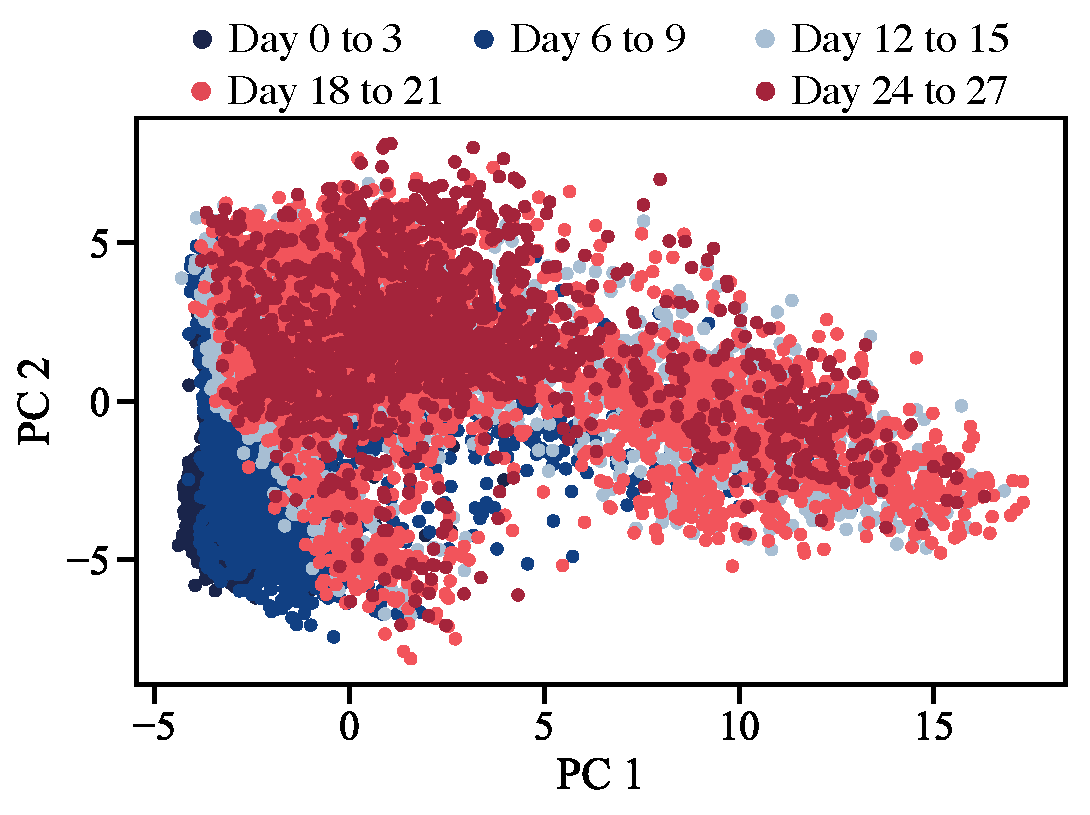
\includegraphics[width=.5\linewidth, valign=t]{figures/fig_data_moon_days_full.pdf}}
    \subfloat[\centering PCA embedding of the embryoid body scRNA-seq data colored by the lineage branch class.]{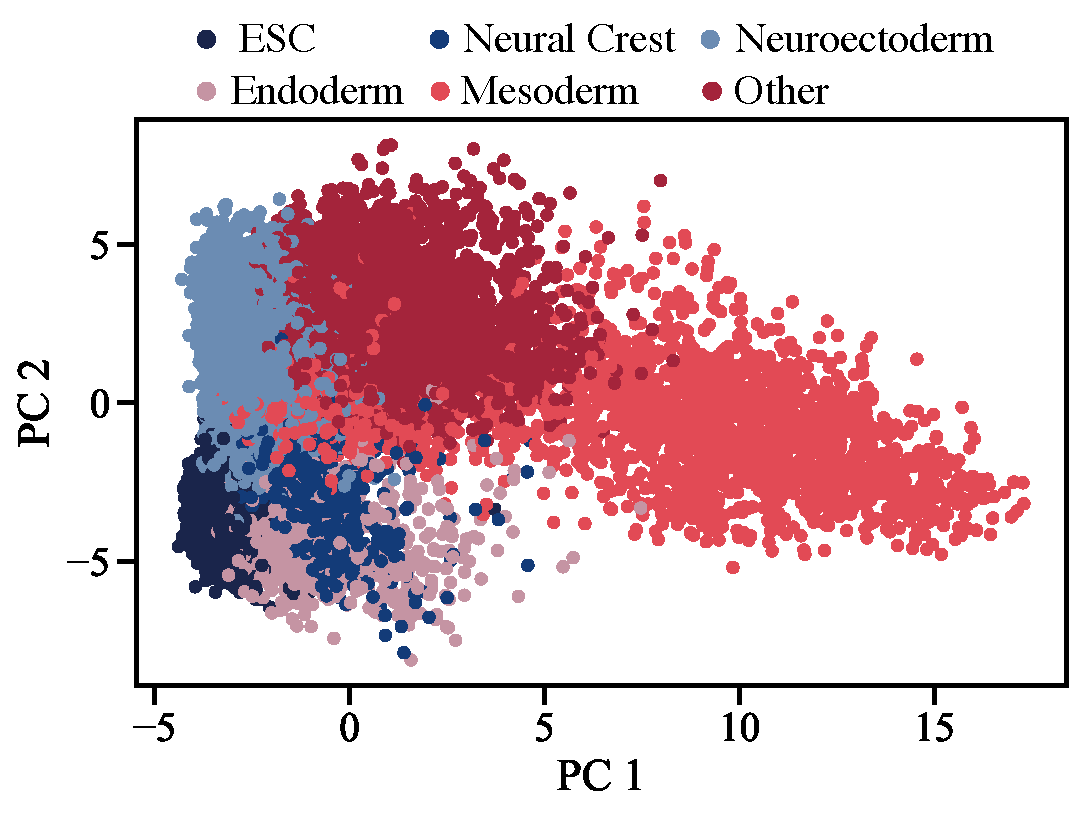
\includegraphics[width=.5\linewidth, valign=t]{figures/fig_data_moon_Branches_full.pdf}}
\end{minipage}\hfill
\begin{minipage}{0.39\linewidth}
    \subfloat[\centering Distribution of cell lineage branch classes in the data or  predicted by \textsc{JKOnet} or the forward method.]{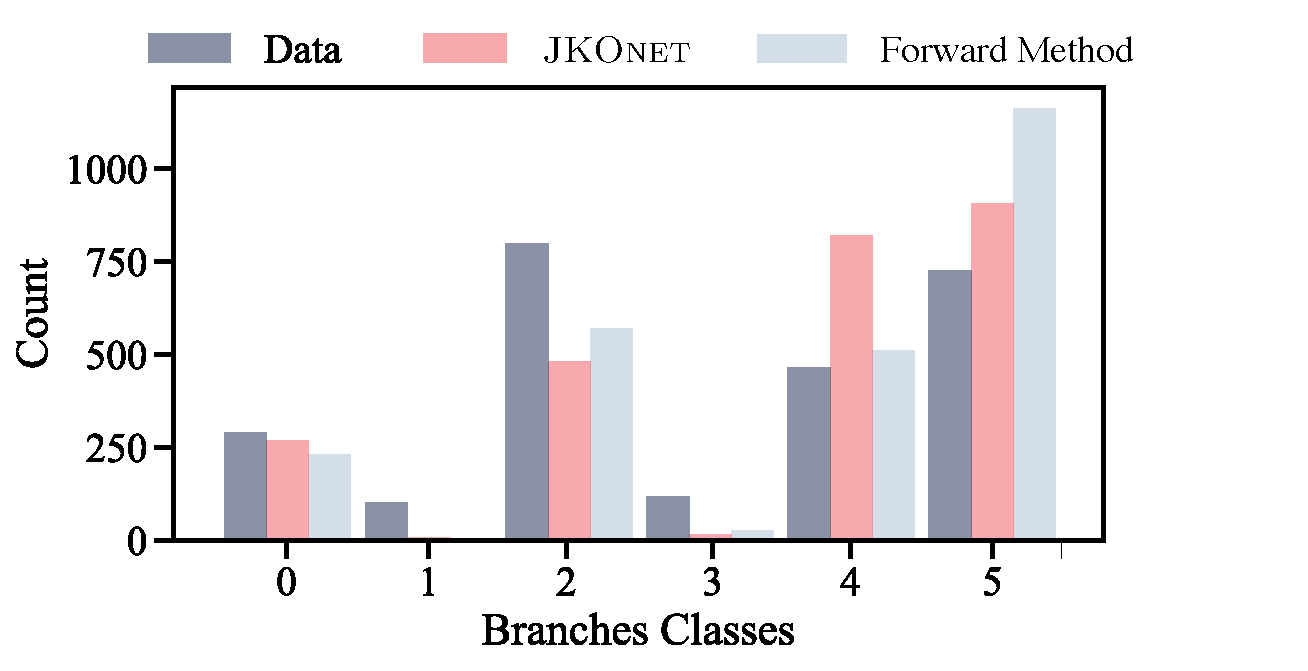
\includegraphics[width=.9\linewidth, valign=t]{figures/fig_distribution_cell_types_Branches.pdf}}
\end{minipage}\hfill

\begin{minipage}{0.58\linewidth}
    \subfloat[\centering PCA embedding of \textsc{JKOnet} predictions colored by the snapshot time.]{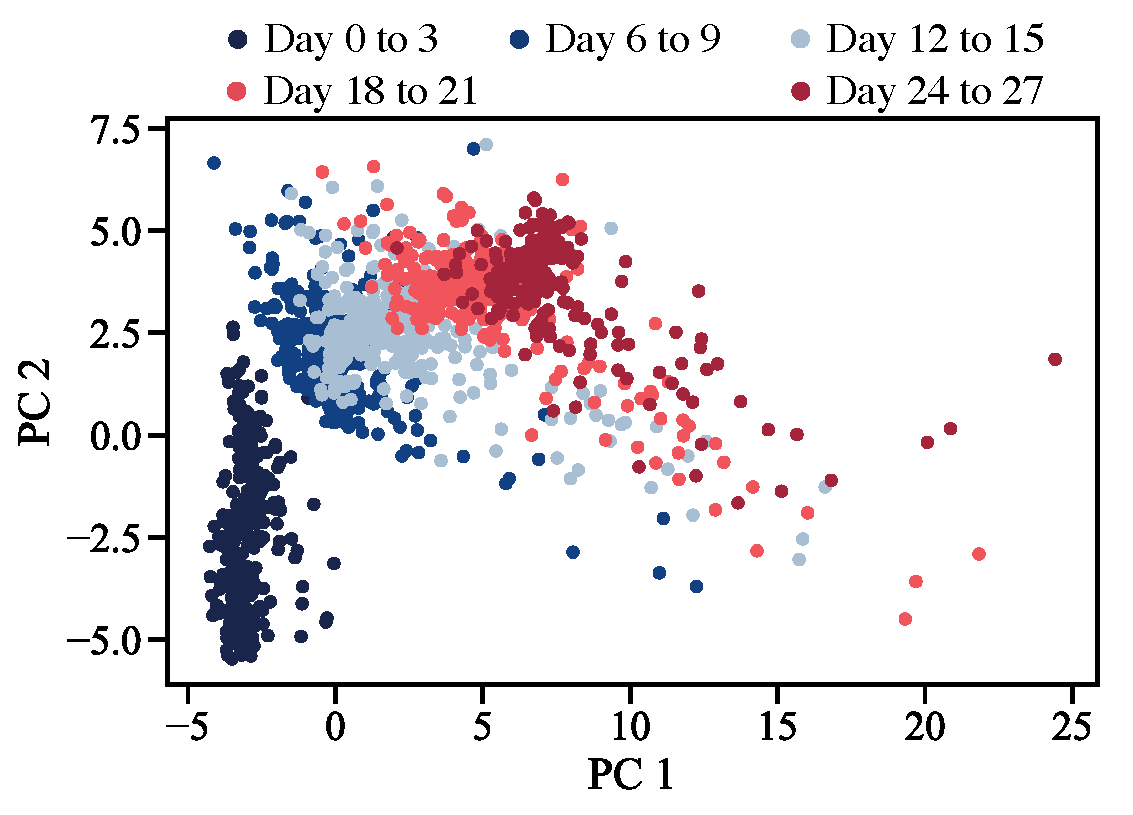
\includegraphics[width=.5\linewidth, valign=t]{figures/fig_implicit_moon_pred_days.pdf}}
    \subfloat[\centering  PCA embedding of \textsc{JKOnet} predictions colored by the lineage branch class.]{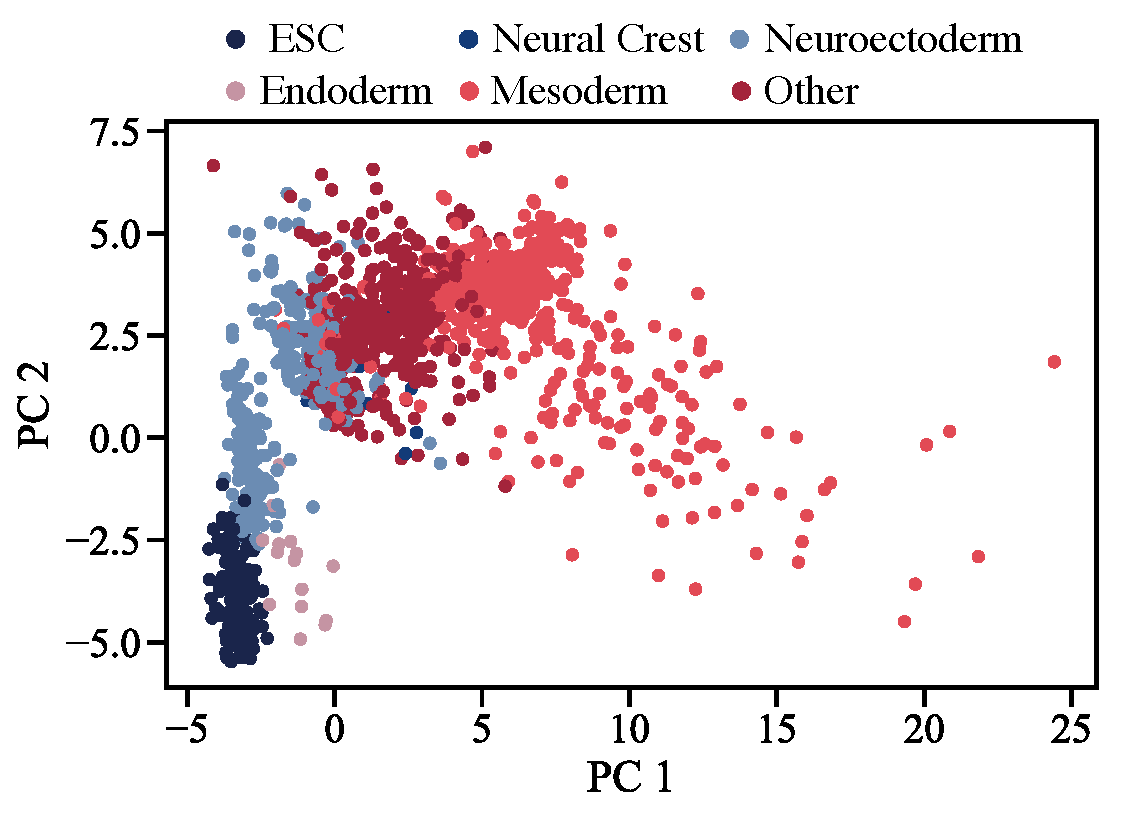
\includegraphics[width=.5\linewidth, valign=t]{figures/fig_implicit_moon_pred_Branches.pdf}}
    \captionof{figure}{Analysis of population dynamics predictions of \textsc{JKOnet} on the embryoid body scRNA-seq data.}
    \label{fig:exp_jkonet_cell}
\end{minipage}\hfill
\begin{minipage}{0.39\linewidth}


\captionof{table}{Evaluation of cell lineage branch classification performance of \textsc{JKOnet} and the forward method on the embryoid body scRNA-seq data based on the $\ell_1$-distance of the histograms and the Hellinger distance $H^2$ \eqref{eq:hellinger} of the predicted branch class distributions (using 3 runs).}
\label{tab:exp_jkonet_cell_class}
\centering
	\resizebox{\linewidth}{!}{%
    \begin{tabular}{lcc}
    \toprule
         \textbf{Method} & \multicolumn{2}{c}{\textbf{Cell Lineage Classification}} \\
         & $\ell_1$ & $H^2$ \\
    \midrule
    \textbf{One-Step Ahead} \\
        \tabindent Forward Method & $132.27 \pm 5.00$ & $0.026 \pm 0.002$ \\
        \tabindent \textsc{JKOnet} & $\bf{88.80 \pm 0.57}$ & $\bf{0.016 \pm 0.001}$ \\
    \textbf{All-Steps Ahead} \\
        \tabindent Forward Method & $\bf{185.47 \pm 12.18}$ & $0.033 \pm 0.002$ \\
        \tabindent \textsc{JKOnet} & $215.60 \pm 12.53$ & $0.034 \pm 0.004$ \\
    \bottomrule
    \end{tabular}
}
\end{minipage}
\end{table*}

We investigate the ability of \textsc{JKOnet} to predict the evolution of cellular and molecular processes through time.
The advent of single cell profiling technologies has enabled the generation of high-resolution single-cell data, making it possible to profile individual cells at different states in the development. 
A key difficulty in learning the evolution of cell populations is that a cell is (usually)  destroyed during a measurement. Thus, although one is able to collect features at the level of individual cells, the same cell cannot be measured twice. Instead, we collect independent samples at each snapshot, resulting in \emph{unaligned} distributions across snapshots, without access to ground-truth single-cell trajectories. 
The goal of learning individual dynamics is to identify ancestor and descendant cells, and get a better understanding of biological differentiation or reprogramming mechanisms. 

We apply \textsc{JKOnet} to embryoid body single-cell RNA sequencing (scRNA-seq) data \citep{moon2019}, describing the differentiation of human embryonic stem cells grown as embryoid bodies into diverse cell lineages over a period of 27 days. During this time, cells are collected at 5 different snapshots (day 1 to 3, day 6 to 9, day 12 to 15, day 18 to 21, day 24 to 27) and measured via scRNA-seq (resulting in 15,150 cells). For details on the dataset and data preprocessing see \S~\ref{app:cell_dataset}.
We run \textsc{JKOnet} as well as the baseline on the first 20 components of a principal component analysis (PCA) of the 4000 highly differentiable genes (see Fig.~\ref{fig:moon_expl_variance}).
We split the dataset into train and test data ($\sim 15 \%$) and parameterize both energy $J_\xi$ and ICNN $\psi_\theta$ with linear layers ($\epsilon = 1.0$, $\tau = 1.0$, \S~\ref{app:hyperparam}).

\paragraph{Capturing Spatio-Temporal Dynamics.}
Given the samples from the cell population at day 1 to 3 ($\mu_0$), \textsc{JKOnet} learns the underlying spatio-temporal dynamics giving rise to the developmental evolution of embryonic stem cells. 
As no ground truth trajectories are available in the data, we use distributional distances, i.e., the entropy-regularized Wasserstein distance $W_\varepsilon$ \eqref{eq:reg-ot} \citep{flamary2021pot}, to measure the correctness of the predictions at each time step.
We hereby measure the $W_\varepsilon$ discrepancy between data and predictions for one-step ahead as well as inference of the entire evolution (all-steps ahead) for each time step $t_i$, see results in Table~\ref{tab:exp_jkonet_cell_pred}. \textsc{JKOnet} outperforms the forward method in terms of $W_\varepsilon$ \eqref{eq:reg-ot} distance for both one-step ahead and all-steps ahead predictions for all time steps. 
The performance of both methods is relatively stable even until day 24 to 27, i.e., the $W_\varepsilon$ distance does not significantly grow for future snapshots.
We further visualize the first two principal components of the entire dataset (Fig.~\ref{fig:exp_jkonet_cell}a) and of \textsc{JKOnet}'s predictions on the test dataset ($\sim 500$ cells per snapshot, Fig.~\ref{fig:exp_jkonet_cell}d). Visualization of predictions of the forward method can be found in the Appendix (Fig.~\ref{fig:exp_forward_cell}a). 

\paragraph{Capturing Biological Heterogeneity.}
Besides measuring the ability of \textsc{JKOnet} to model and predict the spatio-temporal dynamics of embryonic stem cells, we would like to guarantee, at a more macroscopic level, that \textsc{JKOnet} is also able to learn the cell's differentiation into various cell lineages.
Embryoid bodies differentiation covers key aspects of early embryogenesis and thus captures the development of embryonic stem cells (ESC) into the mesoderm, endoderm, neuroectoderm, neural crest and others.

Following \citet[Fig. 6, Suppl. Note 4]{moon2019}, we compute lineage branch classes (Fig.~\ref{fig:moon_analysis}c) for all cells based on an initial $k$-means clustering ($k=30$) in a 10-dimensional embedding space using PHATE, a non-linear dimensionality reduction method capturing a denoised representation of both local and global structure of a dataset (Fig.~\ref{fig:moon_analysis}b).
For details, see \S~\ref{app:lineage_analysis}.
We then train a $k$-nearest neighbor ($k$-NN) classifier ($k=5$) to infer the lineage branch class based on a 20-dimensional PCA embedding of a cell (classes: ESC: 0, neural crest: 1, neuroectoderm: 2, endoderm: 3, mesoderm: 4, other: 5).

We analyze the captured lineage branch heterogeneity of the population predicted by \textsc{JKOnet} and the forward method by estimating the lineage branch class of each cell using the trained $k$-NN classifier. The predicted populations colored by the estimated lineage branch as well as the data with the true lineage branch labels are visualized in Figure~\ref{fig:exp_jkonet_cell}e and Figure~\ref{fig:exp_jkonet_cell}b, respectively.
The corresponding predicted and true distributions of lineage branch classes are shown in Figure~\ref{fig:exp_jkonet_cell}c.
To quantify how well \textsc{JKOnet} and the forward method capture  different cell lineage branches, we compute the $\ell_1$ distance between the  predicted and true histograms as well as the Hellinger distance 
\begin{equation} \label{eq:hellinger}
    H^2(a, b)=\frac{1}{2} \sum_{i=1}^{k}\left(\sqrt{a_{i}/\|a\|_1}-\sqrt{b_{i}/\|b\|_1}\right)^{2}
\end{equation}
between both true and predicted class discrete distributions $a$ and $b$.
Figure~\ref{fig:exp_jkonet_cell}c and Table~\ref{tab:exp_jkonet_cell_class} demonstrate that both, \textsc{JKOnet} and the forward method, capture most lineage branches during the differentiation of embryonic stem cells. Both methods, however, have difficulties recovering cells of the neural crest (class 1) and the endoderm (class 3), lineage branches which are scarcely represented in the original data. 
The analysis further suggests that both methods reduce in performance w.r.t. biological heterogeneity when predicting the entire trajectory (all-steps ahead), instead of inferring the next snapshot only (one-step ahead).


\section{Discussion}
We proposed \textsc{JKOnet}, a model to infer and predict the evolution of population dynamics using a proximal optimal transport scheme, the JKO flow.
\textsc{JKOnet} solves local JKO steps using ICNNs and learns the energy that parameterizes these steps by fitting JKO flow predictions to observed trajectories using a fully differentiable bilevel optimization problem.
We validate its effectiveness through experiments on synthetic potential- and trajectory-based population dynamics, and observe that it is far more robust to noise than a more direct Forward approach. We use \textsc{JKOnet} to infer the developmental trajectories of human embryonic stem cells captured via high-dimensional and time-resolved single-cell RNAseq. 
Our analysis also shows that \textsc{JKOnet} captures diverse cell fates during the incremental differentiation of embryonic cells into multiple lineage branches.
Using proximal optimal transport to model real complex population dynamics thus makes for an exciting avenue of future work. Extensions could include modeling higher-order interactions among population particles in the energy function, e.g., cell-cell communication.
